\documentclass[aip,jcp,reprint,amsmath,amssymb]{revtex4-1}

\usepackage[pdftex]{graphicx}
\usepackage[]{threeparttable}

\newcommand{\mt}[1]{\boldsymbol{\mathbf{#1}}}           % matrix symbol
\newcommand{\vt}[1]{\boldsymbol{\mathbf{#1}}}           % vector symbol
\newcommand{\tr}[1]{#1^\text{t}}                        % transposition
\newcommand{\diff}[2]{\dfrac{\partial #1}{\partial #2}} % partial derivative

\newcommand{\sn}{\text{sn}}                             % Jacobi function sn
\newcommand{\cn}{\text{cn}}                             % Jacobi function cn
\newcommand{\dn}{\text{dn}}                             % Jacobi function dn

\newenvironment{smallarray}[1]                          % small arrays
{\null\,\vcenter\bgroup\scriptsize
	\renewcommand{\arraystretch}{1.5}
	\arraycolsep=.13885em
	\hbox\bgroup$\left[\array{@{}#1@{}}}
{\endarray\right]$\egroup\egroup\,\null}

\begin{document}

\title{A Simplified Formulation for Molecular Dynamics with Rigid Bodies}

\author{Ana J. Silveira}
\email{asilveira@plapiqui.edu.ar}
\affiliation{Planta Piloto de Ingenier\'ia Qu\'imica, PLAPIQUI, Universidad Nacional del Sur, Camino La Carrindanga Km 7-CC: 717, Bah\'ia Blanca, Argentina}

\author{Charlles R. A. Abreu}
\email{abreu@eq.ufrj.br}
\affiliation{Chemical Engineering Department, Escola de Qu\'imica, Universidade Federal do Rio de Janeiro, Rio de Janeiro, RJ 21941-909, Brazil}

\date{\today}

\begin{abstract}
In Molecular Dynamics, sets of atoms collectively behaving as rigid bodies are often used to model entire molecules or parts thereof. Such a coarse-graining strategy eliminates degrees of freedom and admits larger time steps without abandoning the atomistic character of a model. In this paper, we rely on a particular factorization of the rotation matrix to simplify the mechanics of systems containing rigid molecules. Then, we present equations of motion and devise time-reversible, measure-preserving integrators for both microcanonical (NVE) and canonical (NVT) dynamics. We also develop new expressions for computing the virial pressure of rigid-body systems under periodic boundary conditions. Finally, simulations of liquid water are employed to analyze the numerical aspects of the proposed methodology.
\end{abstract}

\maketitle


\section{Introduction}
\cite{Omelyan_2011} multiple time scale md for fluids with orientational dof. canonical and isokinetic ensembles.
systematic errors
\begin{itemize}
\item[1] Kamberaj\cite{Kamberaj2005}\cite{Yan_2008,Akimov_2012,Geiger_2013} \cite{Aimoli_2014}
assumption equipartition of the kinetic energy between the translational and rotational degrees of freedom. We demonstrate that this assumption is not valid and it dramatically affects the drift.
to our knowledge, have not been reported in the
order of the operators
\item[2] our paper review
\item[3] coarse grained: 
Along with advances in software and hardware, improvements in molecular dynamics (MD) algorithms have allowed researchers to extend both the time and the length scales attainable in atomistic simulations. This progress has fomented the ambitious attempt of elucidating complex physical phenomena such as the mechanisms underlying molecular motors, pathways for nanoparticle assembly, and interfacial phenomena, to name just a few. Because of its complexity and large computational demand, such a challenging task requires strategies to enlarge the achievable scales even further. One of the strategies employed to speed up MD simulations is the suppression of unimportant degrees of freedom, as might be the case of intramolecular vibrations. Iterative methods such as SHAKE\cite{Ryckaert1977} and RATTLE\cite{Andersen1983} achieved this suppression by adding constraints to the equations of motion. This is the standard approach in the common case of molecular models with fixed bond lengths and bending angles, but flexible dihedral angles. However, for molecules modeled as rigid structures or those containing rigid substructures,\cite{Miller2002} the dynamics of rigid bodies emerges as a suitable approach. This is expected to be computationally more efficient because the constraints are treated implicitly. In addition, and most importantly, it is possible to devise symplectic integrators for simulations in the microcanonical ensemble. Being symplectic implies phase-space volume preservation and time reversibility, which are sufficient conditions for numerical integrators to be used in hybrid Monte Carlo (HMC) methods.\cite{Duane1987} In this context, Miller \textit{et al}.\cite{Miller2002} have introduced a symplectic integrator for the rotational motion represented in terms of unit quaternions. This approach has been successfully employed in plain MD as well as in HMC methods to simulate a wide variety of systems composed of rigid molecules, including liquid water,\cite{Sakamaki2011, Reinhardt2012, Palmer2014, Gonzales2014} ice,\cite{Geiger2014} hydrates,\cite{Tribello2009, Gorman2012} gases diffusing in metal-organic frameworks,\cite{Ghoufi2010} and so forth. It has also been applied for molecules designed as collections of interconnected rigid bodies, which is a coarse-graining strategy used for proteins,\cite{Terada2003}, molecular machines,\cite{Akimov2008, Konyukhov2010} nanoparticles,\cite{Knorowski2012, Patra2013} etc.

\end{itemize}

In this paper, we report formulation for the motion of rigid bodies in the microcanonical (NVE) and canonical (NVT) ensembles, as well as numerical integrators for both cases. Our contribution in the NVE case resides on a factorization of the rotation matrix that allows a Hamiltonian formalism to be devised without the need of extending the rotational phase space, thus simplifying the formulation of Miller \textit{et al}.\cite{Miller2002} In the NVT case, both the translational and rotational degrees of freedom are simultaneously coupled to a unique Nos\'e-Hoover chain (NHC) thermostat. This differs from the approach of Kamberaj \textit{et al}.,\cite{Kamberaj2005} in which two thermostat chains act separately on the rotational and the translational degrees of freedom. We also simplify the calculation of pressure for systems with rigid bodies whose constituent atoms interact via a pairwise potential under periodic boundary conditions. For this, we derive two alternative expressions: one that depends exclusively on the resultant interaction forces between body pairs and one that corrects the pressure calculated in terms of interactions among freely moving atoms.

The paper is organized as follows. In Sec.~\ref{sec:molecular_dynamics}, we devise numerical integrators for both the NVT dynamics, whose performance and correctness we assess in Sec.~\ref{sec:numerical_results}. Moreover, we analyze the statistical distributions of the sampled energies in the NVT case, and check the equation we developed for computing pressure. Finally, we present some concluding remarks in Sec.~\ref{sec:conclusion}.

\subsection{Microcanonical Ensemble: A Review}
algebraic manipulations
Prompted by the introduction of a particular factorization of the rotational matrix, in a previous paper\cite{Abreu_2017} we reformulated the Hamiltonian equations of motion for rigid bodies, from which we obtained symplectic integrators in the microcanonical (NVE) ensemble.
Nos\'{e}-Hoover chain thermostat. the non-symplectic character, we used the approximate solution for rotation, as we high quality and non-Hamiltonian dynamics admitos no backward error analyisis. We now will briefly review the key expressions of the metioned paper. First, recall that the translational and rotational degrees of freedom are decoupled. Mathematicaly, the position of a particle $j$,  constituent of a rigid body, will vary with time as $\vt r_j(t) = \vt r(t) + \tr{[{\mt A}(\vt q(t))]}\vt d_j$, where $\vt r(t)$ is the position of the center of mass of the body, $\tr{\mt A(\vt q(t))}$ is obtained by transposing the rotational matrix and $\vt d_j$ is the position of the particle in the body-fixed frame of reference. Note that unit quaternions $\vt q = \tr {[\begin{array}{cccc} q_1 & q_2 & q_3 & q_4 \end{array}]}$ are employed to represent the orientations of rigid bodies, which satisfy the known relation\cite{Goldstein2002} $\tr{\vt q}{\vt q} = \|\vt q\|^2 = q_1^2 + q_2^2 + q_3^2 + q_4^2 = 1$, as well as $\tr{\vt q}{\vt q} = 0$.
The matrix $\mt A$ is computed from a given unit quaternion $\vt q$ by\cite{Allen1989,Miller2002}
\begin{equation*}
\label{eq:A_from_q}
\mt A(\vt q) = \begin{smallarray}{ccc}
q_1^2 + q_2^2 - q_3^2 - q_4^2 & 2(q_2 q_3 + q_1 q_4) & 2(q_2 q_4 - q_1 q_3) \\
2(q_2 q_3 - q_1 q_4) & q_1^2 - q_2^2 + q_3^2 - q_4^2 & 2(q_3 q_4 + q_1 q_2) \\
2(q_2 q_4 + q_1 q_3) & 2(q_3 q_4 - q_1 q_2) & q_1^2 - q_2^2 - q_3^2 + q_4^2  
\end{smallarray},
\end{equation*}
which admits the following factorization:
\begin{equation}
\label{eq:factorization_of_A}
{\mt A} = \tr{\mt B}{\mt C}.
\end{equation} 
that depend on the quaternion components as
\begin{equation}
\label{eq:def_B_and_C}
\mt B(\vt q) = \begin{smallarray}{rrrr}
-q_2 & -q_3 & -q_4 \\
 q_1 & -q_4 &  q_3 \\
 q_4 &  q_1 & -q_2 \\
-q_3 &  q_2 &  q_1
\end{smallarray}
\; \text{and} \;
\mt C(\vt q) = \begin{smallarray}{rrrr}
-q_2 & -q_3 & -q_4 \\
 q_1 &  q_4 & -q_3 \\
-q_4 &  q_1 &  q_2 \\
 q_3 & -q_2 &  q_1
\end{smallarray}.
\end{equation}
Note that both $\mt B$ and $\mt C$ depend linearly on the Euler parameters, which makes Eq.~\eqref{eq:factorization_of_A} aconvenient factorization of matrix $\mt A$. This factorization provides a relation between the three-dimensional angular velocity vector $\vt \omega$ and the four-dimensional rates of change of the quaternion components, which is
\begin{equation}
\label{eq:relation_qdot_omega}
\dot{\vt q} = \frac{1}{2} \mt B \vt \omega.
\end{equation}
It avoids the use of an ficticious angular velocity component, as Miller~\textit{et al.}\cite{Miller2002}. An important feature of this relation is that it preserves the unit-norm constraint of a quaternion upon infinitesimal rotation. Note that, for simplicity, we might omit the argument of a matrix-valued function (like $\mt A$, $\vt B$, or $\mt C$) when such argument is $\vt q$. 

For a three-dimensional system consisting of $N$ non-collinear rigid bodies that interact via a potential $U(\vt r, \vt q)$, we define the Hamiltonian in terms of its generalized coordinates ($\vt r_i$ and $\vt q_i$) and conjugate momenta ($\vt p_i$ and $\vt \pi_i$), and kinetic energy as follows:

\begin{equation}
\label{eq:H_NVE}
\mathcal{H} = U(\vt r,\vt q) + \sum_{i=1}^N \left(\frac{\tr{\vt p}_i{\vt p}_i}{2m_i} + \frac{\tr{\vt \pi}_i {\mt B}_i {\mt I}_i^{-1} \tr{\mt B}_i {\vt \pi}_i}{8}\right),
\end{equation}

The equations of motion are obtained from the Hamiltonian by $\dot{\vt r} = \partial \mathcal{H} / \partial \vt p$, $\dot{\vt p} = -\partial \mathcal{H} / \partial \vt r$, $\dot{\vt q} = \partial \mathcal{H} / \partial \vt \pi$, and $\dot{\vt \pi} = -\partial \mathcal{H} / \partial \vt q$.\cite{Goldstein2002}. some algebra manipulations where we defined $\mt \Omega = \mt B(\vt \pi)$, it follows that $\tr{\mt B}{\vt \pi} = - \tr{\mt \Omega}{\vt q}$. For a rigid body composed of $n_p$ individual particles, the derivative $\partial U/\partial \vt r$ is obtained by
\[
\diff{U}{\vt r} = -\vt F = -\sum_{j=1}^{n_p} {\vt F_j},
\]
where $\vt F_j$ is the force applied on particle $j$, expressed in the space-fixed frame of reference and thus $\vt F$ is the resultant force on the body. As demonstrated in Abreu, we have
\[
\diff{U}{\vt q} = -2 \mt C \vt \tau = -2 \mt C \sum_{j=1}^{n_p} {\vt \delta_j} \times {\vt F_j},
\]
where $\vt \tau$ is the resultant torque exerted on the body, also expressed in the space-fixed frame. e. Finally, after carrying out the required differentiations of $\mathcal{H}$  and substituting $\tr{\mt B} \vt \pi = - \tr{\mt \Omega} \vt q = 2 {\mt I} \vt \omega$, we obtain the following Hamiltonian system of equations of motion for a rigid body:
\begin{subequations}
\label{eq:EDO_system}
\begin{align}
&\dot{\vt r} = \frac{1}{m} \vt p \\
&\dot{\vt p} = \mt F \\
&\dot{\vt q} = \frac{1}{2} \mt B \vt \omega \label{eq:EDO_q} \\
&\dot{\vt \pi} = \frac{1}{2} \mt \Omega \vt \omega + 2 \mt C \vt \tau \label{eq:EDO_pi}
\end{align}
\end{subequations}

we now consider the entries of $\vt \omega$ individually. Given that $2{\mt I}{\vt \omega} = \tr{\mt B}{\vt \pi}$, according to Eq.~\eqref{eq:vector_entries}, each entry of $\vt \omega$ is obtained by
\begin{equation}
\label{eq:omega_entry}
\omega_k = \frac{\tr{\vt \pi} \hat{\mt B}_k \vt q}{2 I_k},
\end{equation}
where $\hat{\mt B}_k$ is one of the permutation matrices presented in Appendix~\ref{sec:auxiliary_math}. In this context, the Hamiltonian of the rigid body can be rewritten as
\begin{equation}
\label{eq:H_split_omega}
\mathcal{H} = \frac{\tr{\vt p} \vt p}{2m} + U(\vt r, \vt q) + \frac{1}{2} \sum_{k=1}^3 I_k \omega_k^2.
\end{equation}

Finally, we open the products $\mt B \vt \omega$ and $\mt \Omega \vt \omega$ as in Eq.~\eqref{eq:product_B_vector}, which leads us to the following new form for the equations of motion in Eqs.~\eqref{eq:EDO_q} and \eqref{eq:EDO_pi}:
\begin{subequations}
\label{eq:EDO_system_alternative}
\begin{align}
&\dot{\vt q} = \frac{1}{2} \left( \sum_{k=1}^3 \omega_k \hat{\mt B}_k \right) \vt q \label{eq:edo_q} \\
&\dot{\vt \pi} = \frac{1}{2} \left( \sum_{k=1}^3 \omega_k \hat{\mt B}_k \right) \vt \pi + 2 \mt C \vt \tau \label{eq:edo_pi}
\end{align}
\end{subequations}

where an index $i$ ranging from $1$ to $N$ indicates the quantities related to each body, with $m_i$ is the mass and  $\mt I_i$ the inertia tensor which in the principal frame is a diagonal matrix withe entries given by ($I_1$,$I_2$,$I_3$). 


The phase space of the whole system contains $3N$ spatial coordinates and $4N$ quaternion components, along with their $7N$ conjugate momenta. Of course, $2N$ implicit constraints are known to exist, as $\tr{\vt q}_i{\vt q}_i = 1$ and $\tr{\vt q}_i{\vt \pi}_i = 0$ for all $i$. A Hamiltonian dynamics in phase space will have $\mathcal{H} = E$ as an integral of motion. The dynamics of this system is governed by a Liouville operator with individual operators defined as
\[
\begin{split}
i\!L_b &= \sum_{i=1}^N \left( \tr{\vt F}_i \diff{}{\vt p_i} + 2 \tr{\vt \tau}_i \tr{\mt C}_i \diff{}{\vt \pi_i} \right), \\
i\!L_t &= \sum_{i=1}^N \frac{\tr{\vt p}_i}{m_i}\diff{}{\vt r_i}, \quad \text{and} \\
i\!L_k &= \frac{1}{2} \sum_{i=1}^N {\omega_i}_k \left( \tr{\vt q}_i\tr{\hat{\mt B}_k} \diff{}{\vt q_i} + \tr{\vt \pi_i}\tr{\hat{\mt B}_k} \diff{}{\vt \pi_i} \right).
\end{split}
\]

Therefore, a symplectic integrator can be devised using a splitting scheme with the action of each propagator (boost, free translation, and free uniaxial rotation) occurring simultaneously for all rigid bodies in the system. If there are no external forces acting on the bodies, then additional conserved quantities are the total linear momentum $\sum_{i=1}^N \vt p_i = \vt P$ and the generator of infinitesimal Galilean boosts\cite{Ray1999, Schwichtenberg2015} $\sum_{i=1}^N(\vt p_i t - m_i \vt r_i) = \boldsymbol{\mathcal G}$. If periodic boundary conditions are employed, as it is usual in molecular dynamics simulations, then there is no rotational symmetry and, consequently, no conservation of the total angular momentum.

By defining $i\!L_r = \sum_{k=1}^3 i\!L_k$ for a complete free rotation, the Liouville operator corresponding to the original case of Eq.~\eqref{eq:EDO_system} (as best noticed in its alternative form, Eq.~\eqref{eq:EDO_system_alternative}) can be written as
\begin{equation}
\label{eq:full_operator_uniaxial}
i\!L = i\!L_t + i\!L_b + i\!L_r,
\end{equation}
where $i\!L_t$ corresponds to the first term in the right-hand of Eq.~\eqref{eq:tras_rot_op}. The factorization we employ here for the Liouville operator in Eq.~\eqref{eq:full_operator} is
\begin{equation}
\label{eq:trotter_splitting_NVE}
e^{\Delta t i\!L_{NVE}} = e^{\frac{\Delta t}{2} i\!L_b} e^{\Delta t i\!L_r} e^{\Delta t i\!L_t} e^{\frac{\Delta t}{2} i\!L_b}.
\end{equation}

Update of forces and torques is required only after the free translation and free rotation have been carried out. Following Miller \textit{et al}.,\cite{Miller2002} each complete rotation is split as
\begin{equation}
\label{eq:splitting_rot}
e^{\Delta t i\!L_r} = \prod_{j=1}^n \left( e^{\frac{\delta t}{2} i\!L_3} e^{\frac{\delta t}{2} i\!L_2} e^{\delta t i\!L_1} e^{\frac{\delta t}{2} i\!L_2} e^{\frac{\delta t}{2} i\!L_3} \right),
\end{equation}
where ${\delta t} = {\Delta t}/n$. This means that free rotation, which is computationally inexpensive for not involving force calculations, can be carried out with a smaller time step for accuracy improvement.


\subsection{Canonical Ensemble}
\label{sec:canonical}

Knowledge about the dynamics and statistical mechanics of non-Hamiltonian systems has advanced considerably in recent years.\cite{Tuckerman_1999, Tuckerman2001, Sergi2001, Sergi2003, Ezra2004, Sergi2004, Ezra2006, Sergi2010b} In this context, invaluable tools have been devised for the development and analysis of simulation methods based on the concept of extended phase space. Sergi and Ferrario\cite{Sergi2001} describe a simple way of systematically generating conservative trajectories in an arbitrary phase space. If vector $\vt x$ represents a phase-space point, $H(\vt x)$ is a scalar field, and $\boldsymbol{\mathcal B}(\vt x)$ is a matrix-valued function, then the equation of motion
\begin{equation} \label{eq:eq_of_motion}
\dot{\vt x} = \boldsymbol{\mathcal B}\diff{H}{\vt x}
\end{equation}
will generate a flow that conserves the value of $H$, provided that $\boldsymbol{\mathcal B}$ is skew-symmetric (that is, $\tr{ \boldsymbol{ \mathcal B }} = -\boldsymbol{ \mathcal B }$). A generalized Liouville operator can then be defined as\cite{Sergi2004}
\[
i\!L = \tr{\dot{\vt x}}\diff{}{\vt x} = \tr{\left(\diff{H}{\vt x}\right)} \tr{\boldsymbol{\mathcal B}} \diff{}{\vt x}.
\]

The system might exhibit a non-vanishing phase-space compressibility $\kappa(\vt x) = \sum_j \partial \dot{x}_j/\partial x_j$ if any variable in $\vt x$ affects its own time-derivative. According to Tuckerman and coworkers,\cite{Tuckerman_1999, Tuckerman2001} although the phase-space volume element $d\vt x$ is no longer conserved, there exits an invariant measure $e^{-w(\vt x)}d\vt x$, where $w(\vt x)$ is the indefinite time integral of $\kappa(\vt x)$. Using the generalized Liouville operator, such relation between $\kappa$ and $w$ can be written as
\begin{equation}
\label{eq:relation_kappa_w}
\kappa = \dot w = i\!L w.
\end{equation}

We employ the technique of Sergi and Ferrario\cite{Sergi2001} to couple a single Nos\'e-Hoover chain\cite{Martyna1992} (NHC) composed of $M$ thermostats to a system of $N$ rigid bodies. This is simpler than the approach of Kamberaj \textit{et al}.,\cite{Kamberaj2005} who employed two thermostat chains independently coupled to the translational and rotational degrees of freedom. To this end, we consider extra coordinates $\eta_j$ and their conjugate momenta $p_{\eta_j}$, for $j$ ranging from $1$ to $M$. The conserved ``extended Hamiltonian'' in this case is
\begin{equation}
\label{eq:H_nvt}
H = \mathcal{H}(\vt r,\vt p,\vt q,\vt \pi) + \sum_{j=1}^{M}\frac{p_{\eta_j}^2}{2Q_j} + L k_b T\eta_1 + k_b T\sum_{j=2}^M \eta_j,
\end{equation}
where $\mathcal H$ is the same as in Eq.~\ref{eq:H_NVE}, $k_b T$ is the Boltzmann constant multiplied by the system temperature, $L$ is a constant to be determined, and each $Q_j$ is an inertial parameter of thermostat $j$. As recommended in Ref.~\onlinecite{Martyna1992}, one can make $Q_1 = L k_b T t_d^2$ and $Q_j = k_b T t_d^2$ for $j \geq 2$, where $t_d$ is a characteristic time scale of the system. The equations of motion regarding generalized coordinates are identical to those of a Hamiltonian system, i.e. $\dot{\vt r}_i = {\partial H}/{\partial \vt p_i}$ and $\dot{\vt q}_i = {\partial H}/{\partial \vt \pi_i}$ for every particle $i$ and $\dot{\eta}_j = {\partial H}/{\partial {p_\eta}_j}$ for every thermostat $j$. However, the equations of motion for generalized momenta contain non-Hamiltonian terms. For instance, the first thermostat of the chain acts on the translational and rotational momenta of each particle $i$ as
\[
\begin{split}
\dot{\vt p}_i &= -\diff{H}{\vt r_i} - {\vt p}_i \diff{H}{p_{\eta_1}} \quad \text{and} \\
\dot{\vt \pi}_i &= -\diff{H}{\vt q_i} - {\vt \pi}_i \diff{H}{p_{\eta_1}}.
\end{split}
\]

In the right-hand side of each equation above, the first term fulfills the skew-symmetry condition with respect to the corresponding coordinate while the second term enacts the coupling with the mentioned thermostat. In turn, the equation of motion for $p_{\eta_1}$ must contain terms to ensure skew-symmetry with respect to the equations already shown, along with a term regarding the action of a second thermostat. The result is
\[
{\dot p}_{\eta_1} = \sum_{i=1}^N \left( \tr{\vt p_i} \diff{H}{\vt p_i} + \tr{\vt \pi_i} \diff{H}{\vt \pi_i}\right) - \diff{H}{\eta_1} - p_{\eta_1} \diff{H}{p_{\eta_2}}.
\]

Each additional thermostat will then act on the preceding one, and be acted upon by the succeeding one. Therefore, for $j$ from $2$ to $M-1$, the equations of motion are
\[
{\dot p}_{\eta_j} = -\diff{H}{\eta_j} + p_{\eta_{j-1}} \diff{H}{p_{\eta_{j-1}}} - p_{\eta_j} \diff{H}{p_{\eta_{j+1}}}.
\]

Finally, as the last thermostat will just act on the previous one, its equation of motion can be obtained by simply replacing $j = M$ and removing the last term in the equation above. Therefore, if we take all the required derivatives (including those described in Sec.~\ref{sec:hamiltonian}), the equations of motion for a system of rigid bodies coupled to a single Nos\'e-Hoover chain become
\begin{subequations}
\label{eq:nhc_system}
\begin{align}
&\dot{\vt r}_i = \frac{{\vt p}_i}{m_i} \\ 
&\dot{\vt p}_i = {\vt F}_i - \alpha_1 \vt p_i \label{eq:nhc_p} \\
&\dot{\vt q}_i = \frac{1}{2} \mt B_i \vt \omega_i \label{eq:nhc_q} \\
&\dot{\vt \pi}_i = \frac{1}{2} \mt \Omega_i \vt \omega_i + 2 \mt C_i \vt \tau_i - \alpha_1 \vt \pi_i \label{eq:nhc_pi} \\
&\dot{\eta}_j = \alpha_j \label{eq:nhc_eta} \\
&{\dot p}_{\eta_j} = G_j - \alpha_{j+1} p_{\eta_j}  \label{eq:nhc_p_eta}
\end{align}
\end{subequations}

In the equations above, ${\vt \omega}_i = \frac{1}{2} {\mt I}_i^{-1} \tr{\mt B}_i {\vt \pi}_i$, $\alpha_j = {p_{\eta_j}}/{Q_j}$ for $j \leq M$ and $\alpha_{M+1} = 0$, while
\begin{align*}
&G_1 = \sum_{i=1}^N \left( \frac{\tr{\vt p}_i{\vt p}_i}{m_i} + \tr{\vt \omega}_i \mt I_i \vt \omega_i \right) - L k_b T \quad \text{and}\\
&G_j = \frac{p_{\eta_{j-1}}^2}{Q_{j-1}} - k_b T \qquad \text{for} \; j > 1.
\end{align*}

Note that the $3N$ momentum components in Eq.~\ref{eq:nhc_p}, the $4N$ components in Eq.~\ref{eq:nhc_pi}, and the thermostat momenta in Eq.~\ref{eq:nhc_p_eta} affect their own time-derivatives. Thus, the thermostatted system has a phase-space compressibility $\kappa = -7N \alpha_1 - \sum_j \alpha_{j+1}$. Resorting to Eq.~\ref{eq:nhc_eta} and the fact that $\alpha_{M+1} = 0$, the function $w(\vt x)$ that determines the invariant phase-space measure is given by
\begin{equation}
\label{eq:nhc_measure}
w = -7N \eta_1 - \sum_{j=2}^M \eta_j.
\end{equation}

Finally, analysis of the probability distribution generated by the canonical equations of motion can be carried out via the generalized phase-space analysis of Tuckerman \textit{et al}.\cite{Tuckerman2001} For this, conservation laws must be identified and driven variables must be eliminated. For a system without external forces, the extended energy $H$ and the vector quantity $e^{\eta_1}\sum_{i=1}^N {\vt p}_i = \vt K$ are integrals of motion, while the center-of-mass position can be considered as a driven variable.\cite{Tuckerman2001} Moreover, $2N$ equations must be eliminated from the system due to the constraints involving $\vt q_i$ and $\vt \pi_i$ for all $i$. In the general case, by taking all these facts into account and applying the analysis of Ref.~\onlinecite{Tuckerman2001}, we can deduce that the metric determinant factor of the effective phase space is $\sqrt{g} = e^{(6N-2) \eta_1 + \sum_{j=2}^M \eta_j}$ and that the correct canonical distribution is attained if one makes $L = 6N$. In the particular (and rather common) situation in which one sets $\vt P = \vt 0$ at the beginning of a simulation, one must make $L = 6N - 3$ because all three elements of $\vt P$ will be conserved.\cite{Martyna1994}

\subsection{Reversible, Measure-Preserving Integration of the Canonical Equations of Motion}

As in the Hamiltonian case, the evolution of a phase-space function $f(\vt r, \vt p, \vt q, \vt \pi, \vt \eta,{\vt p}_\eta)$ is given by the relation $f(t) = e^{t i\!L}f_0$, but now in the context of the generalized Liouville theorem.\cite{Tuckerman_1999, Tuckerman2001} Thus, we can employ the Trotter-Suzuki splitting to devise a time-reversible algorithm for integrating the equations of motion. In the microcanonical case, each separate term of the Liouville operator is Hamiltonian and, therefore, each factor of the splitting is a symplectic propagator. As a result, the whole propagator is symplectic and thus preserves the phase-space volume element. It is widely recognized that this property is important for numerical stability.\cite{Skeel1997} In the case of non-Hamiltonian systems, Ezra\cite{Ezra2006} introduced a systematic method for deriving accurate integrators which are not only time-reversible, but also preserve the phase-space measure associated with the original equations of motion. In short, a factorization scheme will preserve a given measure $e^{-w(\vt x)}d\vt x$ if each individual propagator preserves the same measure. As the author has shown,\cite{Ezra2006} for a particular splitting $i\!L = \sum_k i\!L^{(k)}$, measure preservation will take place if $\sum_j \tfrac{\partial}{\partial x_j} [e^{-w(\vt x)}\dot{x}_j^{(k)}] = 0$ for all $k$. Here, $\dot{\vt x}^{(k)}$ refers to the system of equations obtained from the individual operator $i\!L^{(k)}$, which might display its own compressibility $\kappa^{(k)} = \sum_j \partial \dot{x}_j^{(k)}/\partial x_j$. By means of the product rule, it is straightforward to devise an equivalent but more meaningful criterion, which is
\begin{equation}
\label{eq:split_kappa_w}
\kappa^{(k)} = i\!L^{(k)} w.
\end{equation}

Therefore, if the function $w(\vt x)$ that derives from Eq.~\ref{eq:relation_kappa_w} also satisfies Eq.~\ref{eq:split_kappa_w} for all $k$, then the corresponding factorization will preserve the measure $e^{-w(\vt x)}d\vt x$. Here, we propose and compare two distinct measure-preserving integrators for a rigid-body system coupled to a single thermostat chain. In the first one, the generalized Liouville operator is written as $i\!L = i\!L_\text{NVE} + i\!L_\text{NHC}$, where $i\!L_\text{NVE}$ is defined as in Eq.~\ref{eq:full_operator} and, as it follows from Eq.~\ref{eq:nhc_system},
\begin{equation}
\label{eq:iL_NHC}
\begin{split}
i\!L_\text{NHC} = &-\alpha_1 \sum_{i=1}^N \left( \tr{\vt p}_i \diff{}{\vt p_i} + \tr{\vt \pi}_i \diff{}{\vt \pi_i}\right) + \\
&+ \sum_{j=1}^{M} \left[\alpha_j \diff{}{\eta_j} + (G_j - \alpha_{j+1} p_{\eta_j}) \diff{}{p_{\eta_j}}\right].
\end{split}
\end{equation}

Then, by retaining the NVE factorization presented in Eq.~\ref{eq:trotter_splitting_NVE}, we write the full exponential operator for each time step as
\begin{equation}
\label{eq:trotter_splitting_NHC}
e^{\Delta t i\!L} = e^{\frac{\Delta t}{2} i\!L_\text{NHC}} e^{\frac{\Delta t}{2} i\!L_b} e^{\Delta t i\!L_r} e^{\Delta t i\!L_t}  e^{\frac{\Delta t}{2} i\!L_b} e^{\frac{\Delta t}{2} i\!L_\text{NHC}}.
\end{equation}

The Nos\'e-Hoover chain propagator is further split by making $i\!L_\text{NHC} = \sum_{j=0}^M i\!L_\text{NHC}^{(j)}$ and, afterwards,
\[
e^{\frac{\Delta t}{2} i\!L_\text{NHC}} = \Pi_{j=1}^n \Bigg[ \prod_{j=M}^1 e^{\frac{\Delta t}{4} i\!L_\text{NHC}^{(j)} } \Bigg] e^{\frac{\Delta t}{2} i\!L_\text{NHC}^{(0)} } \Bigg[ \prod_{j=1}^M e^{\frac{\Delta t}{4} i\!L_\text{NHC}^{(j)} } \Bigg].
\]

The boost, translation, and rotation propagators already satisfy the criterion in Eq.~\ref{eq:split_kappa_w} with the function $w$ expressed in Eq.~\ref{eq:nhc_measure} (they are all incompressible and keep $w$ unchanged). The NHC propagator is further split into factors that also satisfy Eq.~\ref{eq:split_kappa_w}.




In order to satisfy the criterion in Eq.~\ref{eq:split_kappa_w} for all factors, given the function $w$ expressed in Eq.~\ref{eq:nhc_measure}, we further split the NHC contribution as $i\!L_\text{NHC} = \sum_{j=0}^M i\!L_\text{NHC}^{(j)}$, where
\begin{subequations}
\begin{align}
i\!L_\text{NHC}^{(0)} &= -\alpha_1 \sum_{i=1}^N \left( \tr{\vt p}_i \diff{}{\vt p_i} + \tr{\vt \pi}_i \diff{}{\vt \pi_i}\right) + \alpha_1 \diff{}{\eta_1}, \\
i\!L_\text{NHC}^{(j)} &= (G_j - \alpha_{j+1} p_{\eta_j}) \diff{}{p_{\eta_j}} + \alpha_{j+1} \diff{}{\eta_{j+1}}, \label{eq:iL_NHC_j} \\
i\!L_\text{NHC}^{(M)} &= G_M \diff{}{p_{\eta_M}},
\end{align}
\end{subequations}
with $j$ varying from $1$ to $M-1$ in Eq.~\ref{eq:iL_NHC_j}. Then, each propagator $e^{\frac{\Delta t}{2} i\!L_\text{NHC}}$ present in Eq.~\ref{eq:iL_NHC} is factorized as
\[
e^{\frac{\Delta t}{2} i\!L_\text{NHC}} = \Bigg[ \prod_{j=M}^1 e^{\frac{\Delta t}{4} i\!L_\text{NHC}^{(j)} } \Bigg] e^{\frac{\Delta t}{2} i\!L_\text{NHC}^{(0)} } \Bigg[ \prod_{j=1}^M e^{\frac{\Delta t}{4} i\!L_\text{NHC}^{(j)} } \Bigg].
\]

The action of the propagator $e^{t i\!L_\text{NHC}^{(0)}}$ is the solution of the equations $\dot{\vt p}_i = -\alpha_1 \vt p_i$ and $\dot{\vt \pi}_i = -\alpha_1 \vt \pi_i$ for all $i \in [1,N]$ and $\dot{\eta}_1 = \alpha_1$, with all other variables remaining constant at their initial values. This system can be solved analytically, which results in
\begin{align*}
&\vt p_i(t) = \vt p_i^0 e^{-\alpha_1 t} \\
&\vt \pi_i(t) = \vt \pi_i^0 e^{-\alpha_1 t} \\
&\eta_1(t) = \eta_1^0 + \alpha_1 t
\end{align*}

In turn, the propagator $e^{t i\!L_\text{NHC}^{(j)}}$ defined in Eq.~\ref{eq:iL_NHC_j} behaves according to the equations $\dot{p}_{\eta_j} = G_j - \alpha_{j+1} p_{\eta_j}$ and $\dot{\eta}_{j+1} = \alpha_{j+1}$, with all variables other than $p_{\eta_j}$ and $\eta_{j+1}$ kept unchanged, whose analytical solution is
\begin{align*}
&p_{\eta_j}(t) = p_{\eta_j}^0 + \Big( G_j - \alpha_{j+1} p_{\eta_j}^0 \Big) \phi\left(\alpha_{j+1} t\right) t \\
&\eta_{j+1}(t) = \eta_{j+1}^0 + \alpha_{j+1} t
\end{align*}
where $\phi(x) = (1-e^{-x})/x$. We might note that, in order to avoid numerical issues with $x \rightarrow 0$, we evaluate $\phi(x)$ as $\sum_{n=0}^3 {(-1)^n x^n}/{(n+1)!}$ whenever $|x| \leq 10^{-4}$. The solution above is equivalent to that found in Ref.~\onlinecite{Martyna1996}.

Finally, the propagator $e^{t i\!L_\text{NHC}^{(M)}}$ involves a unique differential equation $\dot{p}_{\eta_M} = G_M$, whose solution is
\[
p_{\eta_M}(t) = p_{\eta_M}^0 + G_M t.
\]

------------

The second splitting scheme we propose here relies on the definition of the operator
\begin{align*}
i\!L_b^\ast &= \sum_{i=1}^N \left( \tr{\vt F}_i - \alpha_1 \tr{\vt p}_i \right) \diff{}{\vt p_i} \\
&+ \sum_{i=1}^N \left(2 \tr{\vt \tau}_i \tr{\mt C}_i - \alpha_1 \tr{\vt \pi}_i \right) \diff{}{\vt \pi_i} + \alpha_1 \diff{}{\eta_1}.
\end{align*}



It is worth noting that an analytical solution can also be derived for the system of equations $\dot{\vt p}_i = {\vt F}_i - \alpha_1 \vt p_i$ and $\dot{\vt \pi}_i = 2 \mt C_i \vt \tau_i - \alpha_1 \vt \pi_i$ for all $i \in [1,N]$ if all other variables are constant. These equations are equivalent in form to the one solved above, so that their solutions are
\begin{align*}
&{\vt p}_i(t) = {\vt p}_i^0 + \left({\vt F}_i - \alpha_1 {\vt p}_i^0 \right) \phi\left(\alpha_1 t \right) t \\
&{\vt \pi}_i(t) = {\vt \pi}_i^0 + \left(2 {\mt C}_i{\vt \tau}_i - \alpha_1 {\vt \pi}_i^0 \right) \phi\left(\alpha_1 t \right) t \\
&\eta_1(t) = \eta_1^0 + \alpha_1 t
\end{align*}


\begin{subequations}
\label{eq:solution_momenta}
\begin{align}
&{\vt p}_i(t) = {\vt p}_i^0 + \left({\vt F}_i - \alpha_1 {\vt p}_i^0 \right) \phi\left(\alpha_1 t \right) t \quad \text{and} \label{eq:solution_p} \\
&{\vt \pi}_i(t) = {\vt \pi}_i^0 + \left(2 {\mt C}_i{\vt \tau}_i - \alpha_1 {\vt \pi}_i^0 \right) \phi\left(\alpha_1 t \right) t. \label{eq:solution_pi}
\end{align}
\end{subequations}

By evaluating these functions simultaneously for all $i$, we accomplish the effect of a propagator $e^{t i\!L_b^\ast}$, where $i\!L_b^\ast$ is the Liouville operator given by
\[
i\!L_b^\ast = \sum_{i=1}^N \left[ \left( \tr{\vt F}_i - \alpha_1 \tr{\vt p}_i \right) \diff{}{\vt p_i} + \left(2 \tr{\vt \tau}_i \tr{\mt C}_i - \alpha_1 \tr{\vt \pi}_i \right) \diff{}{\vt \pi_i} \right].
\]

This is a kind of boost that already incorporates the influence of the thermostat chain. One of the aims of this paper is to compare the performance of the integrator given by Eq.~\ref{eq:trotter_splitting_NHC} to that obtained when the solution in Eq.~\ref{eq:solution_momenta} is considered. For that, we also define a modified Nos\'e-Hoover chain propagator $e^{i\!L^\ast_\text{NHC}}$, as follows:
\begin{equation}
\begin{split}
e^{\frac{\Delta t}{2} i\!L_\text{NHC}^\ast } = &\prod_{j=M}^1 \exp\left[\frac{\Delta t}{4} \left( G_j - \alpha_{j+1} p_{\eta_j} \right) \diff{}{p_{\eta_j}}\right] \\
\times &\exp\left(-\frac{\Delta t}{2} \sum_{j=1}^M \alpha_j \diff{}{\eta_j}\right) \\
\times &\prod_{j=1}^M \exp\left[\frac{\Delta t}{4} \left( G_j - \alpha_{j+1} p_{\eta_j} \right) \diff{}{p_{\eta_j}}\right]
\end{split}
\end{equation}

In the new propagator, $e^{\frac{\Delta t}{2} i\!L_\text{NHC}^{(0)} }$ is removed:
\[
e^{\frac{\Delta t}{2} i\!L_\text{NHC}^\ast} = \Bigg[ \prod_{j=M}^2 e^{\frac{\Delta t}{4} i\!L_\text{NHC}^{(j)} } \Bigg] e^{\frac{\Delta t}{2} i\!L_\text{NHC}^{(1)} } \Bigg[ \prod_{j=2}^M e^{\frac{\Delta t}{4} i\!L_\text{NHC}^{(j)} } \Bigg].
\]

---------
We remark that the integration scheme proposed by Kamberaj \text{et al}.\cite{Kamberaj2005} does not fulfill this criterion. 

Of course, Eqs.~\ref{eq:solution_eta} and \ref{eq:solution_p_eta} are the ones used to evaluate the propagators above. Finally, the complete scheme is
\begin{equation}
\label{eq:modified_splitting}
\begin{split}
e^{\Delta t i\!L} = e^{\frac{\Delta t}{2} i\!L_\text{NHC}^\ast} e^{\frac{\Delta t}{2} i\!L_b^\ast} e^{\Delta t i\!L_r} e^{\Delta t i\!L_t}  e^{\frac{\Delta t}{2} i\!L_b^\ast} e^{\frac{\Delta t}{2} i\!L_\text{NHC}^\ast}.
\end{split}
\end{equation}

 Nevertheless, as will be shown in the forthcoming section, those numerical schemes successfully achieve the specified temperature and an acceptable long-term conservation of the extended energy $H$. Note that the term that premultiplies the extended phase-space volume in the invariant-measure above is a function of $\vt \eta$. Given that the time evolution of the physical variables and the thermostat momenta does not depend on $\vt \eta$, we might conclude that, in this case, the measure-preserving condition for every individual operator can actually be relaxed.


\begin{subequations}
	\label{eq:virial_rigid_bodies}
	\begin{align}
	W &= \frac{1}{3} \sum_{i=1}^{N-1} \sum_{j=i+1}^N \tr{\hat{\vt r}}_{ij} \vt F_{ij} \\
	  &= W_\text{a} - \frac{1}{3} \sum_{i=1}^N \sum_{k=1}^{{n_p}_i} {\tr{\vt \delta}_k}_i {{\vt f}_k}_i,
	\end{align}
\end{subequations}
where $W_\text{a}$ is the atomic virial given by Eq.~\ref{eq:virial_atoms}, while $\vt F_{ij}$ is the total action of body $j$ (and its images) over body $i$ and $\vt f_{ik}$ is the resultant force exerted on the $k$-th atom of body $i$, respectively given by
\
\[
\vt F_{ij} = \sum_{k=1}^{{n_p}_i} \sum_{l=1}^{{n_p}_j} \vt f_{ijkl} \quad \text{and} \quad \vt f_{ik} = \sum_{\substack{j=1\\j \neq i}}^N \sum_{l=1}^{{n_p}_j} \vt f_{ijkl}.
\]

\section{Numerical Results}
\label{sec:numerical_results}

In this section, we analyze some performance aspects of the integration schemes when applied to a molecular system in the liquid state. For this, we simulated a system containing 356 TIP3P water molecules\cite{Price2004} at a density of 999.56 $kg/m^3$. The intermolecular interactions were truncated at 9 \AA. The shifted-force (SF) method\cite{Allen1989, Fennell2006, Toxvaerd_2011} was used to treat both the Coulombic and the 12-6 Lennard-Jones (LJ) interactions.

\subsection{Numerical Stability}
\label{sec:performance}

In order to evaluate the stability of the numerical integrators, we employ a measure given by\cite{Tuckerman2010}
\begin{equation}
\label{eq:performance}
D\!E =  \frac{1}{\mathcal N} \sum_{t=1}^{\mathcal N} \left| \frac{E_t - E_0}{E_0} \right|,
\end{equation}
from which it is possible to quantify the average deviation of the supposedly conserved quantity $E$ (either $\mathcal{H}$ of Eq.~\ref{eq:H_NVE} or $H$ of Eq.~\ref{eq:H_nvt}) from its initial value $E_0$ after a certain number of time steps $\mathcal N$.
It is not the purpose of this work to propose an optimal factorization scheme for the NVT dynamics, but rather to show that a unique thermostat chain is capable of maintaining the average temperature at its specified value while providing the proper sampling of the canonical ensemble. \textbf{In order to use a constant value for the smaller time step in the NHC and NHC* operators $(\Delta t/4)$, we factorized those operators analogously to the scheme given by Eq.~\ref{eq:splitting_rot}}. Recalling that in the NVT dynamics the conserved quantity is the extended energy $H$, in Table~\ref{table:denvt} we show the results of Eq.~\ref{eq:performance} as well as the average temperatures obtained in each case. It can be seen that both integrators, represented by the Eq.~\ref{eq:trotter_splitting_NHC} and Eq.~\ref{eq:modified_splitting}, systematically achieve the specified temperature, regardless of the time step size. In addition, the energy drift is, at its worst, around $1 \%$.

\subsection{New Results}

\begin{table*}
\caption{Results.....}
\label{table:proposed_method}
\begin{ruledtabular}
\begin{tabular}{cccccccc}
$\Delta t$ (fs) & $T$ (K) & $\langle U\rangle$ (kcal/mol) & $\langle K\rangle$ (kcal/mol) & $\langle K_t\rangle$ (kcal/mol) & $\langle K_r\rangle$ (kcal/mol) & P (atm) & $R$ (kcal/mol.ns) \\

\hline
\multicolumn{8}{c}{Proposed Method} \\
1.0 & $300.01\pm0.02$ & $-8465.1\pm0.5$ & $1614.2\pm0.1$ & $807.4\pm0.1$ & $806.8\pm0.1$ & $62\pm2$ & $0.0328$ \\
2.0 & $300.01\pm0.03$ & $-8450.8\pm0.4$ & $1614.2\pm0.2$ & $809.4\pm0.1$ & $804.7\pm0.1$ & $73\pm2$ & $0.597$ \\
3.0 & $299.97\pm0.04$ & $-8425.7\pm0.5$ & $1614.0\pm0.2$ & $812.8\pm0.1$ & $801.2\pm0.2$ & $90\pm2$ & $3.44$ \\
4.0 & $299.93\pm0.04$ & $-8391.4\pm0.6$ & $1613.7\pm0.2$ & $817.1\pm0.2$ & $796.6\pm0.2$ & $119\pm2$ & $5.64$ \\

\hline
\multicolumn{8}{c}{Alternative Method} \\
1.0 & $300.00\pm0.02$ & $-8465.5\pm0.5$ & $1614.1\pm0.1$ & $807.1\pm0.1$ & $807.0\pm0.1$ & $65\pm2$ & $0.108$ \\
2.0 & $299.99\pm0.03$ & $-8450.5\pm0.5$ & $1614.1\pm0.2$ & $809.3\pm0.1$ & $804.7\pm0.1$ & $72\pm2$ & $1.31$ \\
3.0 & $299.98\pm0.04$ & $-8425.9\pm0.5$ & $1614.0\pm0.2$ & $812.5\pm0.1$ & $801.5\pm0.2$ & $88\pm2$ & $2.53$ \\
4.0 & $300.01\pm0.04$ & $-8390.4\pm0.6$ & $1614.2\pm0.2$ & $817.4\pm0.2$ & $796.8\pm0.2$ & $120\pm2$ & $7.31$ \\

\hline
\multicolumn{8}{c}{Method of Kamberaj \textit{et al}.\cite{Kamberaj2005}} \\
1.0 & $299.53\pm0.02$ & $-8470.9\pm0.5$ & $1611.6\pm0.1$ & $806.4\pm0.1$ & $805.2\pm0.1$ & $52\pm2$ & $0.023$ \\
2.0 & $298.24\pm0.03$ & $-8471.2\pm0.5$ & $1604.6\pm0.2$ & $805.4\pm0.1$ & $799.2\pm0.1$ & $47\pm2$ & $17.0$ \\
3.0 & $295.94\pm0.04$ & $-8480.9\pm0.6$ & $1592.3\pm0.2$ & $804.2\pm0.1$ & $788.1\pm0.1$ & $28\pm2$ & $53.2$ \\
4.0 & $292.72\pm0.04$ & $-8494.7\pm0.7$ & $1575.0\pm0.2$ & $802.4\pm0.1$ & $772.5\pm0.2$ & $-1\pm2$ & $60.6$ \\

\hline
\multicolumn{8}{c}{Double-Thermostat Analogue of the Proposed Method} \\
1.0 & $300.00\pm0.02$ & $-8466.0\pm0.5$ & $1614.1\pm0.1$ & $806.6\pm0.1$ & $807.5\pm0.1$ & $60\pm2$ & $6.42$\\
2.0 & $299.98\pm0.03$ & $-8452.0\pm0.5$ & $1614.0\pm0.2$ & $807.1\pm0.1$ & $806.9\pm0.1$ & $71\pm2$ & $80.4$ \\
3.0 & $300.16\pm0.04$ & $-8426.1\pm0.5$ & $1615.0\pm0.2$ & $808.4\pm0.1$ & $806.6\pm0.1$ & $90\pm2$ & $1.38\times10^4$ \\
4.0 & $300.75\pm0.04$ & $-8385.3\pm0.6$ & $1618.2\pm0.2$ & $811.6\pm0.1$ & $806.6\pm0.2$ & $125\pm2$ & $4.29\times10^4$ \\

\hline
\multicolumn{8}{c}{Double-Thermostat Analogue of the Alternative Method} \\
1.0 & $299.98\pm0.02$ & $-8465.6\pm0.5$ & $1614.0\pm0.1$ & $806.6\pm0.1$ & $807.4\pm0.1$ & $56\pm2$ & $4.87$ \\
2.0 & $299.96\pm0.03$ & $-8452.0\pm0.5$ & $1613.9\pm0.2$ & $807.1\pm0.1$ & $806.8\pm0.1$ & $71\pm2$ & $85.1$ \\
3.0 & $300.20\pm0.04$ & $-8426.0\pm0.5$ & $1615.2\pm0.2$ & $808.5\pm0.1$ & $806.7\pm0.1$ & $89\pm2$ & $1.50\times10^4$ \\
4.0 & $300.75\pm0.04$ & $-8384.7\pm0.6$ & $1618.1\pm0.2$ & $811.6\pm0.1$ & $806.6\pm0.2$ & $123\pm2$ & $4.33\times10^4$ \\

\hline
\multicolumn{8}{c}{Single-Thermostat Analogue of the Method of Kamberaj \textit{et al}.\cite{Kamberaj2005}} \\
1.0 & $299.52\pm0.02$ & $-8470.2\pm0.5$ & $1611.6\pm0.1$ & $805.9\pm0.1$ & $805.6\pm0.1$ & $58\pm2$ & $0.272$ \\
2.0 & $298.18\pm0.03$ & $-8471.8\pm0.5$ & $1604.3\pm0.2$ & $804.4\pm0.1$ & $799.9\pm0.1$ & $44\pm2$ & $0.390$ \\
3.0 & $295.97\pm0.04$ & $-8474.6\pm0.5$ & $1592.4\pm0.2$ & $801.6\pm0.1$ & $790.8\pm0.2$ & $29\pm2$ & $3.00$ \\
4.0 & $292.65\pm0.04$ & $-8478.7\pm0.6$ & $1574.6\pm0.2$ & $797.6\pm0.2$ & $777.0\pm0.2$ & $10\pm2$ & $8.12$ \\

\end{tabular}
\end{ruledtabular}
\end{table*}


\begin{table}
	\caption{New results involving Kamberaj \text{et al}.\cite{Kamberaj2005}}
	\label{table:new_results}
	\begin{ruledtabular}
		\begin{tabular}{cccc}
			& \multicolumn{3}{c}{ Temperature (K) } \\
			\cline{2-4}
			$\Delta t$/fs & Proposed & Alternative & Kamberaj \text{et al}. \\
			\hline
			1.0 & $300.01 \pm 0.02$ & $300.00 \pm 0.02$ & $299.52 \pm 0.02$ \\
			2.0 & $300.01 \pm 0.03$ & $299.99 \pm 0.03$ & $298.24 \pm 0.03$ \\
			3.0 & $299.97 \pm 0.04$ & $299.98 \pm 0.04$ & $295.94 \pm 0.04$
		\end{tabular}
	\end{ruledtabular}
\end{table}

\begin{table}
	\caption{New results involving Kamberaj \text{et al}.\cite{Kamberaj2005}}
	\label{table:new_results_2}
	\begin{ruledtabular}
		\begin{tabular}{cccc}
			& \multicolumn{3}{c}{Drift rate [(kcal/mol)/ns]} \\
			\cline{2-4}
			$\Delta t$/fs & Proposed & Alternative & Kamberaj \text{et al}. \\
			\hline
			1.0 & $0.0328$ & $0.108$ & $0.023$ \\
			2.0 & $0.597$  & $1.31$  & $17.0$ \\
			3.0 & $3.44$   & $2.53$  & $53.2$
		\end{tabular}
	\end{ruledtabular}
\end{table}

\subsection{Partition of Energy}
\label{sec:energypartition}

\subsection{Sampling Validation}
\label{sec:samplingvalidation}

In this subsection we present the results from a simple method that serves for checking the consistency between the sampled energy distributions and the theoretical ones. The procedure, introduced and implemented by Shirts ~\cite{Shirts2013}, relies on a quantitative statistical analysis of fitting and it is possible to perform linear and nonlinear fitting or a maximum likelihood approach too. This last approach does not involve any binning of the energies, hence no discretization error is present. We report the results corresponding to that method, and since it is instructive to have a graphical insight, we also show some figures of the linear fitting.

Recall that in the NVT ensemble the probability of observing an energy E is given by
\[
P(E/\beta) = Q(\beta)^{-1}\Omega(E)\exp\left(-\beta E\right),
\]
where $ \beta $ is the Boltzmann's constant, $ \Omega(E) $ is the density of states which does not depend on $ \beta $ , and $ Q(\beta) $  is the canonical partition function, linked to the Helmholtz Free Energy $ (A) $ by $A = -\beta^{-1}\ln(Q)$. 

Taking the ratio of the probability distributions at different temperatures, the unknown density of states cancels out and we get
\begin{equation}
\label{eq:probability_ratio}
\frac{P(E/\beta_2)}{P(E/\beta_1)} = \exp\left[(\beta_2 A_2 - \beta_1 A_1) - (\beta_2 - \beta_1)E\right].
\end{equation}
Taking the logarithm of Eq.~\ref{eq:probability_ratio}, we obtain
\begin{equation}
\label{eq:ln_probability_ratio}
\ln\frac{P(E/\beta_2)}{P(E/\beta_1)} = \left(\beta_2 A_2 - \beta_1 A_1\right) - \left(\beta_2 - \beta_1\right)E.
\end{equation}

The Eq.~\ref{eq:ln_probability_ratio} is the basis for the statistical analysis in the ensemble validation, which determines how many standard deviations the calculated slope is from the specified one,  $ \beta_2 - \beta_1 $. Note that it is independent of the unknown free energies. For a guidance on how to choose the temperature gap the reader is referred to the aforementioned paper. Given that the potential and kinetic energies are separable, the analysis can be made separately as follows

\begin{equation}
\label{eq:probability_ratio_pot}
\frac{P_{pot}(E/\beta_2)}{P_{pot}(E/\beta_1)} = \frac{Q_{pot}(\beta_1)}{Q_{pot}(\beta_2)}  \exp\left[(-\beta_2 - \beta_1)E_{pot}\right]
\end{equation}

\begin{equation}
\label{eq:probability_ratio_kin}
\frac{P_{kin}(E/\beta_2)}{P_{kin}(E/\beta_1)} = \frac{Q_{kin}(\beta_1)}{Q_{kin}(\beta_2)}  \exp\left[(-\beta_2 - \beta_1)E_{kin}\right]
\end{equation}
Furthermore,  it is possible to examine the consistency between the sampled kinetic energy and the corresponding Maxwell-Boltzmann distribution, which is given by the following expression:
\begin{equation}
\label{eq:mb}
P(E_{cin}) = \frac{\beta}{\sqrt{N_{DOF}\pi}} \exp\left[-\frac{\left(\beta E_{kin} - \frac{N_{DOF}}{2}\right)^2}{N_{DOF}} \right],
\end{equation}
where $N_{DOF}$ is the number of degrees of freedom. This last equations is a normal distribution characterized by an average of $ \langle E_{kin} \rangle = (N_{DOF}/2\beta) $ and variance $\sigma^2 = N_{DOF}/2\beta^2$, valid when equipartition of energy is satisfied.

In Fig.~\ref{fig:checkensemble} we show the result from the linear regression analysis for the potential energies sampled using Eq.~\ref{eq:trotter_splitting_NHC}. In figure legends we show the averages temperatures simulated. It can be seen that the mentioned algorithm generates a distribution consistent with the canonical ensemble, and that is also true for the kinetic energies. Likewise, in Fig.~\ref{fig:mbdistribution} we observe a good correspondence between the kinetic energy distribution at $T= 304.99 K$ and the corresponding Maxwell-Boltzmann distribution We arrive at the same conclusions for the approach given by Eq.~\ref{eq:modified_splitting}.

\begin{figure}
	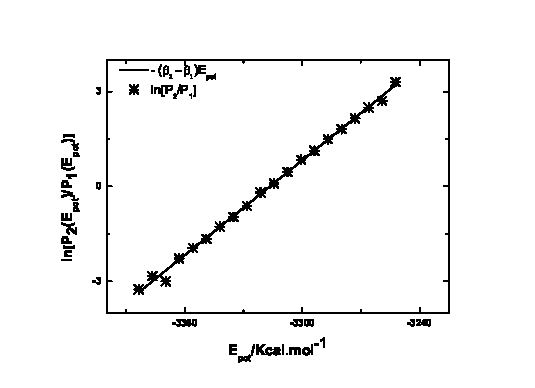
\includegraphics{checkensemble}
	\caption{Linear plot of the log ratio probabilities with the true slope (solid line) and the measured slope from the linear regression analysis (symbols). Simulation of liquid water using Eq.~\ref{eq:trotter_splitting_NHC}, $\Delta t$ = 1~fs, $\bar{T}_1$ = 296.03~K, $\bar{T}_2$ = 304.99~K.}
	\label{fig:checkensemble}
\end{figure}

\begin{figure}
	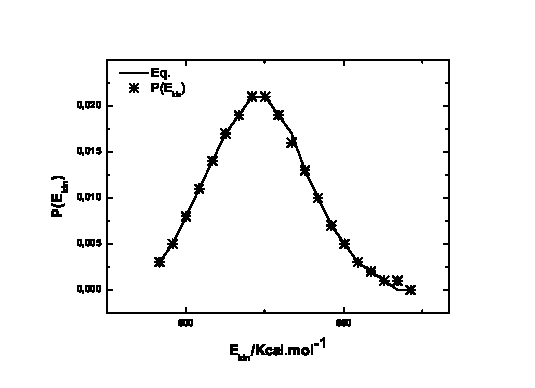
\includegraphics{maxwell-botlzamm-paper}
	\caption{Probability distribution of the kinetic energy with sampled values and those calculated with Eq.~\ref{eq:mb}. Simulation of liquid water using Eq.~\ref{eq:trotter_splitting_NHC}, $\Delta t$ = 1~fs, $\bar{T}$ = 304.99~K.}
\label{fig:mbdistribution}
\end{figure}

Finally, in Table~\ref{table:ensemblevalidation} we present the results of the maximum likelihood approach applied for both NVT integration schemes. It can be seen that the deviations from the true slope, $\Delta T$ = 8.970~K, are less than $1\sigma$. This means that effectively, the sampled values do not deviate from the correct distribution to a statistically noticeable level.

\begin{table}
	\begin{threeparttable}
		\caption{Ensemble Validation of NVT algorithms for liquid water using the Maximum Likelihood Approach \tnote{a} \tnote{b}}
		\label{table:ensemblevalidation}
		\begin{ruledtabular}
			\begin{tabular}{ccccc}
				& \multicolumn{4}{c}{true $\Delta T$ = 8.970 K} \\
				\cline{2-5}
				& \multicolumn{2}{c}{potential} & \multicolumn{2}{c}{kinetic}\\
				\hline
				Method  &$\Delta T/K$ & $\sigma$ dev & $\Delta T/K$ & $\sigma$ dev \\
				\hline % inserts single-line 
				Eq.~\ref{eq:trotter_splitting_NHC} & 9.022 $\pm$ 0.117 & 0.57 & 8.928 $\pm$ 0.051 & 0.63 \\
				Eq.~\ref{eq:modified_splitting}    & 8.965 $\pm$ 0.101 & 0.05 & 8.967 $\pm$ 0.052 & 0.14
		\end{tabular}
		\end{ruledtabular}
		\begin{tablenotes}
			\item[a] The standard deviation of the mean temperature for all cases is $\sigma$ = 0.03.
			\item[b] $\bar{T}_1$ = 296.03~K and $\bar{T}_2$ = 304.99~K.
		\end{tablenotes}
	\end{threeparttable}
\end{table}

%\begin{center}
%  \label{fig:pressure}
%  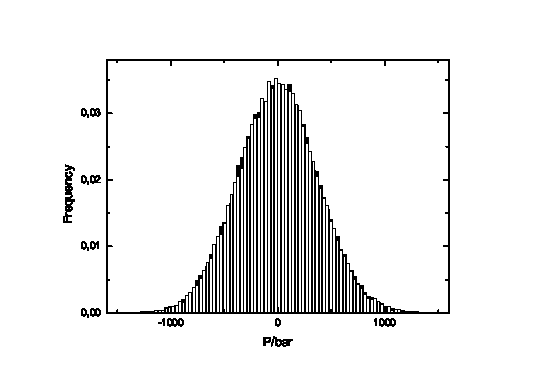
\includegraphics{pressure2}
%  \captionof{figure}{Histograms of pressure obtained in this work (filled bars) and using LAMMPS %(unfilled bars). Simulation of liquid water with NVE integration. $\Delta t : 1 fs$  }
%\end{center}


\section{Concluding Remarks}
\label{sec:conclusion}

\begin{acknowledgments}
The authors acknowledge the financial support provided by Petrobras (project code CENPES 16113).
\end{acknowledgments}

\bibliography{rigid_bodies}
%\begin{table*}
%	\caption{Results with Exact Solution for Free Rotations}
%	\label{table:NVE}
%	\begin{ruledtabular}
%		\begin{tabular}{cccccccc}
%			$\Delta t$ (fs) & $T$ (K) & $\langle U\rangle$ (kcal/mol) & $\langle K\rangle$ (kcal/mol) & $\langle K_t\rangle$ (kcal/mol) & $\langle K_r\rangle$ (kcal/mol) & P (atm) & $R$ (kcal/mol.ns) \\
%			\hline
%			1.0 & $	305.91	\pm	0.03	$ & $	-8395.1	\pm	0.1	$ & $	1645.9	\pm	0.1	$ & $	823.2	\pm	0.1	$ & $	822.7	\pm	0.1	$ & $	146	\pm	2	$ & $0.0456$ \\
%			2.0 & $	305.21	\pm	0.02	$ & $	-8389.5	\pm	0.1	$ & $	1642.1	\pm	0.1	$ & $	823.0	\pm	0.1	$ & $	819.1	\pm	0.1	$ & $	149	\pm	2	$ & $0.656$ \\
%			3.0 & $	304.30	\pm	0.03	$ & $	-8375.4	\pm	0.9	$ & $	1637.2	\pm	0.1	$ & $	824.0	\pm	0.1	$ & $	813.3	\pm	0.1	$ & $	156	\pm	2	$ & $2.87$ \\
%			4.0 & $	304.5	\pm	0.5	$ & $	-8339	\pm	6	$ & $	1638	\pm	3	$ & $	829	\pm	1	$ & $	808.8	\pm	0.6	$ & $	180	\pm	2	$ & $10.1$ \\
%		\end{tabular}
%	\end{ruledtabular}
%\end{table*}

%\begin{table*}
%\caption{Results.....}
%\label{table:NVE}
%\begin{ruledtabular}
%\begin{tabular}{cccccccc}
%$\Delta t$ (fs) & $T$ (K) & $\langle U\rangle$ (kcal/mol) & $\langle K\rangle$ (kcal/mol) & $\langle K_t\rangle$ (kcal/mol) & $\langle K_r\rangle$ (kcal/mol) & P (atm) & $R$ (kcal/mol.ns) \\
%\hline
%1.0 & $305.95\pm0.03$ & $-8395.4\pm0.1$ & $1646.1\pm0.1$ & $823.3\pm0.1$ & $822.9\pm0.1$ & $151\pm2$ & $0.0471$ \\
%2.0 & $305.17\pm0.03$ & $-8389.0\pm0.1$ & $1641.9\pm0.1$ & $823.2\pm0.1$ & $818.8\pm0.1$ & $148\pm2$ & $0.853$ \\
%3.0 & $304.34\pm0.03$ & $-8374\pm2$ & $1637.5\pm0.2$ & $824.0\pm0.1$ & $813.4\pm0.1$ & $152\pm2$ & $3.96$ \\
%4.0 & $303.6\pm0.4$ & $-8349\pm5$ & $1633\pm2$ & $826.8\pm0.2$ & $806.5\pm0.4$ & $168\pm2$ & $8.25$ \\
%\end{tabular}
%\end{ruledtabular}
%\end{table*}
%\begin{table}
%	\begin{threeparttable}
%		\caption{Average deviation of the conserved quantity ($DE$) and average temperatures from liquid water simulation with NVT integration \tnote{a}\tnote{b}}
%		\label{table:denvt}
%		\begin{ruledtabular}
%			\begin{tabular}{ccccc}
%				& \multicolumn{2}{c}{Eq.~\ref{eq:trotter_splitting_NHC}} & \multicolumn{2}{c}{Eq.~%\ref{eq:modified_splitting}} \\
%				\cline{2-5}
%				$\Delta t$/fs & $D\!E$ & $T$/K & $D\!E$ & $T$/K \\
%				\hline
%				1.0 & 0.000043 & 298.16  & 0.000052  & 298.15 \\
%				2.0 & 0.00013  & 298.23  & 0.00017   & 298.06 \\
%				3.0 & 0.00089  & 298.17  & 0.0013    & 298.12
%			\end{tabular}
%		\end{ruledtabular}
%		\begin{tablenotes}
%			\item[a] The standard deviation of the mean temperature for all cases is $\sigma = 0.037$.
%			\item[b] The smaller time step in the NHC and NHC* operators is 0.25 fs.
%		\end{tablenotes}
%	\end{threeparttable}
%\end{table}
\end{document}
